\documentclass[11pt]{article}

\usepackage[T1]{fontenc}
\usepackage[utf8]{inputenc}
\usepackage[english]{babel}
\usepackage[a4paper,margin=1in]{geometry}
\usepackage{microtype}
\usepackage{xcolor}
\usepackage{amsmath,amssymb,amsthm}
\usepackage{mathtools}
\usepackage{booktabs,tabularx}
\usepackage{enumitem}
\usepackage{needspace}
\usepackage{flafter}
\usepackage[section]{placeins}
\usepackage{tikz}
\usetikzlibrary{arrows.meta,positioning}
\usepackage{listings}
\usepackage{hyperref}
\usepackage[nameinlink,noabbrev]{cleveref}

\hypersetup{
  colorlinks=true,
  linkcolor=blue!45!black,
  citecolor=green!40!black,
  urlcolor=blue!55!black,
  pdftitle={A Certificate-Based Branching Analysis for MaxSAT Parameterized by the Number of Clauses},
  pdfauthor={Anonymous author(s)},
  pdfkeywords={MaxSAT, exact algorithms, automated branching analysis, certificates}
}
\emergencystretch=3em
\widowpenalty=1000
\clubpenalty=1000
\lstset{basicstyle=\small\ttfamily,columns=fullflexible,
  keepspaces=true,frame=single,framerule=0.3pt,
  aboveskip=0.7em,belowskip=0.7em}

\newcommand{\MaxSAT}{\textnormal{\textsc{MaxSAT}}}
\newcommand{\OhStar}{O^*}
\newcommand{\OPT}{\operatorname{OPT}}
\newcommand{\anytail}{\mathord{?}}
\newcommand{\plustail}{\mathord{?}^{+}}
\newcommand{\tail}[1]{\mathord{?}_{#1}}
\newcommand{\ntail}[1]{\mathord{?}^{+}_{#1}}

\newtheorem{theorem}{Theorem}
\newtheorem{lemma}[theorem]{Lemma}
\theoremstyle{definition}
\newtheorem{example}{Example}
\theoremstyle{remark}
\newtheorem{remark}[theorem]{Remark}

% SUBMISSION: Retain anonymity or add affiliations as required by the venue.
\title{A Certificate-Based Branching Analysis for \MaxSAT{}
  Parameterized by the Number of Clauses}
% \author{Anonymous author(s)}
\date{}

\begin{document}
\maketitle

\begin{abstract}
We present a pipeline for constructing and checking local branching analyses
for exact \MaxSAT{}. Starting from a partially specified clause neighborhood,
the generator distinguishes empty and nonempty clause tails, exposes further
variables, and searches for branching strategies. It combines assignment
enumeration, removal of dominated alternatives, grouping by variable
substitutions, reductions, and recursive analysis of the resulting formulas.
The output is a certificate recording both the coverage of the case analysis
and the transformations used in each case. A separate checker reconstructs
the refinements, checks local optimum identities, and evaluates branching
inequalities with exact rational arithmetic.

At a fixed target $q$, continuation choices are compared by the weight
$W_q=\sum_i q^{-d_i}$ of their accumulated measure decreases. Its
additivity permits independent continuation selection within each group.
We apply the pipeline to the $(3,2)$-literal bottleneck in the
$\OhStar(1.2886^m)$-time algorithm of~\cite{Xiao2022}, where $m$ is the number of clauses.
Combining generated strategies with branching lemmas from that algorithm, the local
analysis reaches the target $q=1.2872$. We prove the soundness of the certificate rules
and state the conditions under which this local result yields an
$\OhStar(1.2872^m)$-time algorithm. The contribution is a compositional,
machine-checkable analysis pipeline relative to a fixed library of imported
branching lemmas, with the improved local target serving as its case study.
\end{abstract}

\section{Introduction}
\label{sec:introduction}

Exact algorithms for unweighted \MaxSAT{} seek an optimal assignment while
bounding the size of the search needed to find it. The number of clauses
$m$ is a useful measure for this purpose: a branch can be charged for the
clauses it removes, and several consecutive transformations can be analyzed
through their accumulated decreases. The notation $\OhStar$ suppresses
factors polynomial in the input length.

Clause-measure analyses have improved through increasingly detailed treatment
of low-degree variables. Bansal and Raman~\cite{BansalRaman1999} obtained
the bound $\OhStar(1.3413^m)$, Chen and Kanj~\cite{ChenKanj2004} improved
it to $\OhStar(1.3248^m)$, and Xu et al.~\cite{XuEtAl2019} reached
$\OhStar(1.2989^m)$ using resolution and domination. The algorithm
of~\cite{Xiao2022}, which we call the \emph{baseline algorithm}, further
improved the bound to $\OhStar(1.2886^m)$ with polynomial space.
\Cref{tab:history} places our target in this line of results.

\begin{table}[!htbp]
\centering\small
\begin{tabularx}{0.88\linewidth}{@{}lXl@{}}
\toprule
Year & Analysis & Running-time bound \\
\midrule
1999 & Bansal and Raman~\cite{BansalRaman1999} & $\OhStar(1.3413^m)$ \\
2004 & Chen and Kanj~\cite{ChenKanj2004} & $\OhStar(1.3248^m)$ \\
2019 & Xu et al.~\cite{XuEtAl2019} & $\OhStar(1.2989^m)$ \\
2022 & Baseline algorithm & $\OhStar(1.2886^m)$ \\
This work & Certificate-based replacement of Step~5.4 & $\OhStar(1.2872^m)$ \\
\bottomrule
\end{tabularx}
\caption{Selected clause-measure bounds for unweighted \MaxSAT{}.
The last row is the global consequence under the certificate and
imported-result premises of \cref{thm:conditional-global}.}
\label{tab:history}
\end{table}

\subsection{\texorpdfstring{The $(3,2)$-literal bottleneck}{The (3,2)-literal bottleneck}}
\label{sec:bottleneck}

The baseline algorithm applies reductions and branching cases in a fixed
order. Its Step~5 handles a literal $x$ occurring in three clauses and whose
complement occurs in two, with incident clauses
\begin{equation}
 (x\vee C_1)(x\vee C_2)(x\vee C_3)
 (\bar x\vee D_1)(\bar x\vee D_2).
 \label{eq:neighborhood}
\end{equation}
Step~5.4, where $D_1$ and $D_2$ contain only degree-five variables, gives
the limiting branching vector $(6,6,5,5)$.
\Cref{tab:global-vectors} summarizes the baseline cases and identifies
the one we replace. The other cases already meet the target $q=1.2872$:
in particular, $(11,3,3)$ has branching factor approximately
$1.287190881$. Improving Step~5.4 to this target is therefore sufficient
to improve the global bound, provided that the replacement covers the case
and preserves an optimal solution under the baseline algorithm's hypotheses.

\begin{table}[!htbp]
\centering\small
\begin{tabularx}{\linewidth}{@{}lXlr@{}}
\toprule
Step & Literal or case type & Branching vector & Base \\
\midrule
1 & Degree at least six & $(6,1)$ & $1.2852$ \\
2 & $(i,1)$ non-singleton, $i\ge3$ & $(3,3)$ & $1.2600$ \\
3 & Degree three & $(8,1)$ & $1.2321$ \\
4 & Unit-clause case & $(5,2)$ & $1.2366$ \\
5.1 & $(3,2)$, unit-clause case & $(4,2)$ & $1.2721$ \\
5.2 & $(3,2)$ & $(11,3,3)$ & $1.2872$ \\
5.3 & $(3,2)$ & $(6,1)$ & $1.2852$ \\
\textbf{5.4} & \textbf{$(3,2)$ bottleneck} & $\mathbf{(6,6,5,5)}$ & $\mathbf{1.2886}$ \\
5.5 & $(3,2)$ & $(11,10,4,3)$ & $1.2801$ \\
6.1 & $(2,2)$ & $(4,2)$ & $1.2721$ \\
6.2 & $(2,2)$ & $(6,1)$ & $1.2852$ \\
6.3 & $(2,2)$ & $(11,3,3)$ & $1.2872$ \\
6.4 & $(2,2)$ & $(18,18,11,11,11,11,4,4)$ & $1.2870$ \\
7 & $(3,1)$- or $(4,1)$-singletons & Set Cover Problem & $1.2576$ \\
\bottomrule
\end{tabularx}
\caption{Baseline cases, adapted from Table~3 of~\cite{Xiao2022}.
Bases reproduce the source's displayed values; for Step~7 the base is
that of the terminal algorithm. We replace the highlighted Step~5.4 by
a family of local strategies checked at $q=1.2872$.}
\label{tab:global-vectors}
\end{table}

The generator starts from the five-clause neighborhood in
\cref{eq:neighborhood}, with partially specified clause tails. It allows
each tail to be empty, so its root family includes cases covered by neighboring
steps as well as the intended bottleneck. The structural restrictions used
when further variables are exposed come from the ordered baseline algorithm.
The exact root and allowed degrees are given in \cref{sec:configuration};
their coverage of Step~5.4 is established in \cref{sec:global}.

\subsection{Automating a compositional analysis}
\label{sec:motivation}

A good branching rule for an exact algorithm must do two things: preserve an
optimal solution among its children and reduce the instance enough to meet
the desired running-time bound. Both tasks become harder when a useful rule
requires several rounds of branching and reduction. The argument must also
cover every possible local configuration, including configurations whose
clauses contain variables outside the displayed neighborhood.

The bottleneck supplies a concrete setting for automating this analysis:
the target is fixed, the initial neighborhood is small, and the surrounding
algorithm supplies degree restrictions. A useful local strategy may group
assignments by substitutions and then reduce or branch on the residual
formulas. Its quality depends on the composition of all these steps, not
just on the first branching vector. Structural case coverage and recursive
strategy selection must therefore be tracked together.

Our pipeline separates two trees that play different roles. A
\emph{refinement tree} distinguishes possible clause neighborhoods. For each
of its terminal cases, a \emph{strategy tree} describes how to reduce or branch
on an instance in that case. The generator builds these trees from an
analysis script. Within each selected case, it enumerates assignments,
removes dominated choices, groups compatible assignments, and analyzes the
residual formulas. A separate checker reads the resulting trees without
repeating this search.

We select continuations using their weight at the fixed target,
$W_q(v)=\sum_i q^{-d_i}$, where $v=(d_1,\ldots,d_r)$ is the vector of
accumulated clause decreases. A preceding decrease scales this weight by
$q^{-d}$, and recursive alternatives contribute additively. Consequently,
each group can retain its best available continuation independently of
the others; the search then chooses a minimum-weight cover of the remaining
assignments. Ranking continuations by their standalone branching factors
does not have this property, because their weight curves can cross.
\Cref{lem:weight-selection,sec:fixed-target} give the formal argument and
its use in the generator.

The key verification step is simple. For each possible truth-value combination
of the unknown clause tails, the checker computes the best local score before
and after a proposed transformation. The scores must agree after accounting
for the clauses already satisfied. This single test handles reductions and
grouped branches through the same interface. Recurrence bounds are checked
separately from these objective-value identities.

\Needspace{9\baselineskip}
\paragraph{Contributions.}
\begin{enumerate}[leftmargin=1.5em,itemsep=0.25em]
  \item We give a pipeline that combines structural refinement with recursive
    search for local \MaxSAT{} strategies, including assignment dominance,
    substitution-based grouping, and reductions of the resulting children.
    Fixed-target weights permit independent continuation selection and
    minimum-weight selection of possibly overlapping groups.
  \item We define certificate rules for coverage, local transformations, and
    accumulated measure decreases, and prove their compositional soundness.
  \item We apply the pipeline at the rational target $q=1.2872$ and give an
    explicit successful strategy from the generated analysis. We separate
    the generated transformations from the imported results used to derive
    the running-time bound.
\end{enumerate}

\subsection{Related work and positioning}
\label{sec:related}

Automatic branching analysis has a substantial history. Fedin and
Kulikov~\cite{FedinKulikov2004} generated running-time proofs from supplied
simplification rules and reported experiments for SAT, \MaxSAT{}, and
bounded-occurrence \MaxSAT{}. Kulikov~\cite{Kulikov2005} also automated the
discovery of simplification rules and useful splittings for SAT and \MaxSAT{}.
Skjernaa's framework~\cite[Chapter~8]{Skjernaa2004} refines formula patterns,
searches for reductions, and considers branching on variable values and on
whether pairs of variables are equal or different. Thus automatic case
analysis, reduction discovery, and branching beyond individual assignments
are established ideas.

More recently, \v{C}erven\'y and Such\'y~\cite{CervenySuchy2023} generated
parameterized branching algorithms for $d$-Path Vertex Cover. Gao et
al.~\cite{GaoEtAl2024} formulate local branching-rule selection for Maximum
Independent Set as a weighted set-cover problem. These works also motivate
searching for a collection of alternatives rather than choosing a single
branching variable.

Our focus is the integration of clause-tail refinements, recursive analysis
of substitution-generated residual CNFs, and a separate checker for both
coverage and local optimum identities. In particular, the certificate records
actual child formulas and their composition, so a newly added search heuristic
does not require a corresponding heuristic-specific verification rule. We
present this combination for the baseline bottleneck; we do not claim that deeper
search, dominance, or grouping alone is new.

Related resolution techniques appear in
Chen, Xu, and Wang~\cite{ChenXuWang2017}. Other parameterizations, including
those studied by Bliznets and Golovnev~\cite{BliznetsGolovnev2012}, lead to
different bounds. General background on branching recurrences is provided by
Fomin and Kratsch~\cite{FominKratsch2010}.

Finally, proof logging for \MaxSAT{} can certify optimum-preserving
preprocessing, including through the VeriPB and CakePB
systems~\cite{IhalainenEtAl2024}. Our certificate has a different target: a
local case analysis and its recurrence for a family of instances. Its semantic
checks enumerate small local truth tables, while pseudo-Boolean proof logging
supports reasoning about individual, potentially large solver instances.

\paragraph{Organization.}\mbox{}\par
\noindent
\begin{tabularx}{\linewidth}{@{}lX@{}}
\Cref{sec:preliminaries} & Local notation and target weights. \\
\Cref{sec:overview} & Pipeline and worked example. \\
\Cref{sec:certificate} & Certificate rules, composition, and soundness. \\
\Cref{sec:automation} & Automated search and independent checker. \\
\Cref{sec:global} & Generated analysis, global bound, and artifact. \\
\Cref{sec:conclusion} & Conclusion. \\
\Cref{app:normalization,app:script} & Normalization conventions and analysis script.
\end{tabularx}

\section{Preliminaries}
\label{sec:preliminaries}

We use standard unweighted \MaxSAT{} terminology as in~\cite{Xiao2022}.
A formula $F$ is a multiset of clauses: equal clauses are retained with
multiplicity. We assume the normalization described in
\cref{app:normalization}, and write $m=|F|$ and
\[
  \OPT(F)=\max_{\alpha}\operatorname{sat}(F,\alpha),
\]
where $\alpha$ ranges over all assignments and $\operatorname{sat}$ counts
satisfied clauses with multiplicity. We describe transformations of the
optimum directly.
Throughout, $F\uplus G$ denotes multiset union: clause multiplicities add.

A literal $x$ has degree $(i,j)$ if it occurs in $i$ clauses and its complement
$\bar x$ in $j$ clauses. The complementary literal has degree $(j,i)$.
An $(i,1)$-literal is a \emph{singleton} when its unique
negative occurrence is the unit clause $(\bar x)$.

\subsection{Templates, scores, and measure decreases}
\label{sec:local-notation}

A \emph{template} $P$ is a multiset of displayed clauses. It names selected
variables explicitly and uses a \emph{tail} $\anytail$ for the as-yet-undisplayed
part of a clause. A $\plustail$ tail contains at least one literal, whereas a $\anytail$ tail
may be empty. These marks describe clause syntax, not truth values; even a
nonempty tail may evaluate to false. Subscripts distinguish tails, and repeated
identifiers denote the same disjunction. All occurrences of a selected
variable are displayed. Clauses written consecutively form a multiset, so
repeated clauses count separately.

A complete formula \emph{matches} $P$ when it can be written as
$F=P[T]\uplus E$. Here $T$ replaces each tail by a disjunction of literals
on unselected variables, and $E$ contains the remaining clauses.
Even when a clause occurs in both parts, its multiplicities add.
No selected variable occurs in $T$ or $E$. Matching also
respects any degree and singleton restrictions stated for the template.
For a Boolean vector $\tau$ indexed by the tails, define the \emph{local
score}
\begin{equation}
 B_P(\tau)=\max_{\alpha}\operatorname{sat}(P,\alpha,\tau),
 \label{eq:local-score}
\end{equation}
where $\alpha$ assigns the selected variables and each tail is treated as a
Boolean input. A clause made true by a tail counts as one satisfied clause.
Different tails can share hidden variables in a complete instance. Checking
all Boolean vectors $\tau$ includes every realizable combination, and may
therefore reject a valid transformation, but cannot accept an invalid one for
this reason.

A correct branching step produces formulas $F_i$ and nonnegative integer
\emph{offsets} $s_i$ such that
\[
  \OPT(F)=\max_i\bigl(s_i+\OPT(F_i)\bigr).
\]
Its \emph{measure decreases} are $d_i=|F|-|F_i|$. These need not equal the
offsets: an empty false clause contributes to $d_i$ but not to $s_i$.
For example, assigning $x=1$ in $(x)(\bar x)$ gives $s=1$ and $d=2$.
The generator represents such steps locally by transforming templates;
\cref{lem:contextual-replacement} connects a checked local identity to the
corresponding full formulas $F_i$.

\subsection{Fixed-target weights and recurrences}
\label{sec:weights}

For a target $q>1$ and a nonempty integer vector $v=(d_1,\ldots,d_r)$,
define its \emph{fixed-target weight}
\begin{equation}
 W_q(v)=\sum_{i=1}^{r}q^{-d_i}.
 \label{eq:weight}
\end{equation}
Repeated entries are counted separately. A vector of positive integer
decreases is \emph{$q$-admissible} when
\begin{equation}
  W_q(v)\le 1.
  \label{eq:target}
\end{equation}
We use the target $q=1.2872$ and check this inequality
exactly. A local recursive call with no additional decrease has vector $(0)$
and weight one. Such a call can end a continuation after a positive incoming
decrease; by itself it does not establish a progressing recursive step.

\begin{lemma}[Branching recurrence]
\label{lem:recurrence}
Suppose each recursive step has positive decreases satisfying
\cref{eq:target}, and the work at each node, including any intervening
reductions, is polynomial in the input length. Then the running time is
$\OhStar(q^m)$.
\end{lemma}
\begin{proof}
Induction on $m$ bounds the number of leaves by $q^m$: an internal node has
at most $\sum_i q^{m-d_i}\le q^m$ descendant leaves. Each root-to-leaf path
has at most $m$ recursive edges, since every decrease is positive. The number
of nodes is therefore at most $(m+1)q^m$. Polynomial work per node gives
the claimed bound.
\end{proof}

\Needspace{8\baselineskip}
\section{Pipeline overview and a worked example}
\label{sec:overview}

The refinement tree first asks structural questions. Is a chosen tail empty?
If not, which degree can a literal in it have, and where can its other
occurrences lie? Each answer gives a child template. The strategy search then
asks an optimization question: which assignments or groups of assignments
cover an optimal solution with a sufficiently good branching vector?
\Cref{fig:pipeline} shows how the script interleaves them.

\begin{figure}[!htbp]
\centering
\begin{minipage}{0.86\linewidth}
\begin{lstlisting}
frontier <- {root template}
for each command in the analysis script:
    if the command selects a refinement:
        replace selected unresolved templates by their children
    if the command starts a strategy search:
        for each selected unresolved template:
            if a strategy is found, record it and remove the template
require frontier empty
assemble the certificate; check coverage, identities, and vectors
\end{lstlisting}
\end{minipage}
\caption{The generation and checking pipeline. Refinements cover structural
cases; a strategy search resolves cases when it finds a suitable branch or
reduction. The script chooses the refinements and search budgets.}
\label{fig:pipeline}
\end{figure}

\begin{example}[A grouped branch from the certificate]
\label{ex:group}
Consider the following template, obtained by exposing a $(3,1)$-singleton
$y$ in the two negative clauses of the root:
\begin{equation}
\begin{split}
 P={}&(x\vee\tail{1})(x\vee\tail{2})(x\vee\tail{3})\\
     & (\bar x\vee y\vee\tail{4})(\bar x\vee y\vee\tail{5})
       (y\vee\tail{6})(\bar y).
\end{split}
\label{eq:example-parent}
\end{equation}
The four assignments to $(x,y)$ need only two alternatives. The assignments
$(0,0)$ and $(1,0)$ are grouped by fixing $y=0$. When
$y=1$, changing $x$ from $0$ to $1$ cannot lose a satisfied clause: the two
negative $x$-clauses are already satisfied by $y$. Thus $(0,1)$ is dominated
by $(1,1)$.

For the first alternative, let
\[
 H=(x\vee\tail{1})(x\vee\tail{2})(x\vee\tail{3})
   (\bar x\vee\tail{4})(\bar x\vee\tail{5})(\tail{6}).
\]
The unit clause $(\bar y)$ contributes offset~1, and all six clauses of $H$
remain in the recursive formula, including the tail-only clause
$(\tail{6})$. The second alternative satisfies six clauses and falsifies
$(\bar y)$, leaving no local clause. It has offset~6 and decrease~7.
Consequently, for every Boolean tail vector $\tau$,
\begin{equation}
 B_P(\tau)=\max\{1+B_H(\tau),\,6\}.
 \label{eq:example-identity}
\end{equation}
In a complete instance $F=P[T]\uplus E$, the same identity gives
\[
 \OPT(F)=\max\{1+\OPT(H[T]\uplus E),\,6+\OPT(E)\}.
\]
Thus the external clauses remain in both recursive alternatives, including
the alternative with no remaining local clause.
The vector is $(1,7)$, and $q^{-1}+q^{-7}<0.948<1$ at $q=1.2872$.
\end{example}

\begin{figure}[!htbp]
\centering
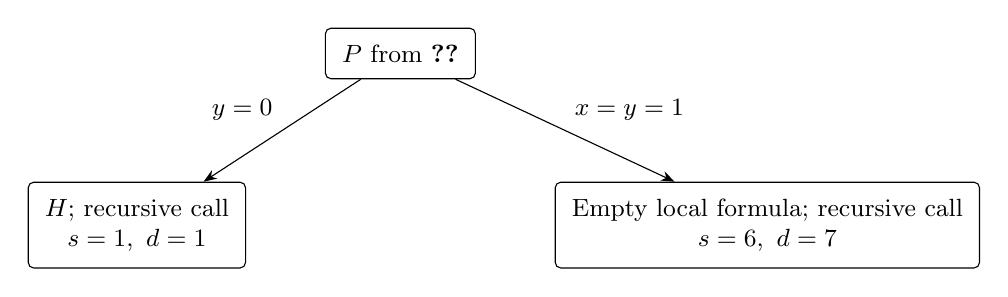
\begin{tikzpicture}[>=Stealth,
 every node/.style={align=center,font=\small},
 case/.style={draw,rounded corners=2pt,inner sep=6pt}]
 \node[case] (p) {$P$ from \cref{eq:example-parent}};
 \node[case,below left=13mm and 10mm of p] (h) {$H$; recursive call\\$s=1,\ d=1$};
 \node[case,below right=13mm and 10mm of p] (e) {Empty local formula; recursive call\\$s=6,\ d=7$};
 \draw[->] (p)--node[above left]{$y=0$}(h);
 \draw[->] (p)--node[above right]{$x=y=1$}(e);
\end{tikzpicture}
\caption{A strategy extracted from the existing certificate, with variable
and tail names relabeled. The external part of the instance remains to be
solved even when the local formula is empty.}
\label{fig:example}
\end{figure}

This example also explains why the generator constructs residual formulas.
A grouped alternative can retain a free variable, so further reductions and
branching can improve its contribution to the final vector. The search can
continue below $H$ instead of treating the group as an indivisible leaf.

\section{Templates and certificate rules}
\label{sec:certificate}

We now formalize the two checks used above: refinements cover the relevant
instances, and strategies preserve their optimum. We use $F$ for a complete
recursive formula and $P$ for its displayed template.

\subsection{Unknown tails and the surrounding formula}

For a strategy transformation, not every tail identifier of the parent need
occur in a child; every identifier that does occur must come from the parent.
The checked score identity justifies any disappearance of local clauses or
tails. Structural refinement has a different role. When a variable is exposed
from a tail, the child's tail describes the remainder after that exposure, and
the displayed fragment may acquire further clauses from $E$. Matching is
always interpreted on the same complete instance, even though its displayed
fragment changes.

The local score $B_P(\tau)$ from \cref{eq:local-score} lets the checker compare
such transformations without constructing a complete formula for each choice
of external clauses.

\subsection{Structural refinements}
\label{sec:refinements}

Refinements distinguish formula structure without making a Boolean assignment.
The two basic operations are shown in \cref{fig:refinement}.

\begin{figure}[!htbp]
\centering
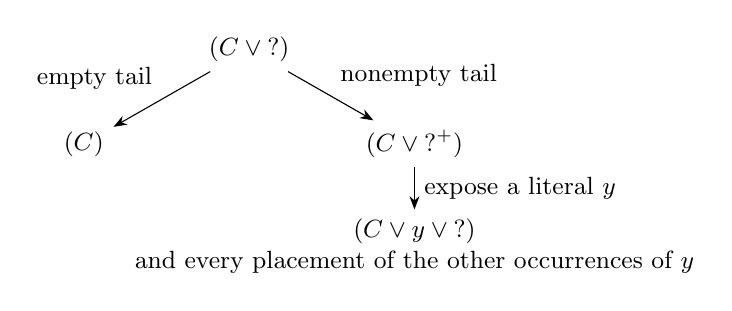
\begin{tikzpicture}[>=Stealth,every node/.style={font=\small,align=center}]
 \node (p) at (0,0) {$(C\vee\anytail)$};
 \node (empty) at (-2.1,-1.2) {$(C)$};
 \node (nonempty) at (2.1,-1.2) {$(C\vee\plustail)$};
 \node (expose) at (2.1,-2.5) {$(C\vee y\vee\anytail)$\\and every placement of the other occurrences of $y$};
 \draw[->] (p)--node[above left]{empty tail}(empty);
 \draw[->] (p)--node[above right]{nonempty tail}(nonempty);
 \draw[->] (nonempty)--node[right]{expose a literal $y$}(expose);
\end{tikzpicture}
\caption{Topological refinement nodes. If $C$ is nonempty, the left child is
an ordinary clause, not an empty clause. After exposing one literal from
$\plustail$, the remaining tail is $\anytail$ and may be empty.}
\label{fig:refinement}
\end{figure}

\paragraph{Tail split.}
Replace a chosen $\anytail$ by the two cases ``empty'' and $\plustail$. These cover every
concrete tail. This is recorded as \texttt{tail\_empty\_or\_nonempty}.

\paragraph{Variable exposure.}
An analysis specifies a finite set of \emph{allowed oriented degrees}
$(i,j)$ for the literal selected from a clause tail. The orientation counts
occurrences of that literal first and its complement second. In our case this
set consists of five classes, listed in \cref{sec:configuration}. Its
completeness follows from the structural assumptions inherited from the baseline
ordered algorithm, not from a bound on clause width.
Choose a literal from a nonempty tail and name it $y$. For each degree in
this set, enumerate all placements of $y$ and $\bar y$ in
existing clause tails, and add clauses for the remaining occurrences.
The selected clause must contain $y$; singleton restrictions fix the unique
negative occurrence to a unit clause. The remaining tail in each affected
clause may be empty. Each concrete occurrence pattern is among these choices,
provided the degree list covers the literals that can be selected.

The format combines a tail split and these exposures in
\texttt{expose\_at\_clause}: an empty child is included for $\anytail$ and omitted
for $\plustail$. Exposure is restricted to templates with distinct, clause-local
single tails. An initial variable declaration constructs the root family;
it is not a refinement of arbitrary formulas.

The coverage requirement can be stated without a separate semantics for
fragments: \emph{every complete instance matching the parent and its
structural restrictions must match at least one child}. Exposing $y$ merely
moves all its occurrences into the displayed fragment of that same instance.
The checker regenerates the child templates, compares them up to renaming,
and rejects missing, extra, or duplicate cases. In format version~2 the
allowed degree list is recorded in the exposure node. Its completeness under
the intended structural restrictions is a mathematical premise, whereas
faithful enumeration of its incidences is checked computationally.

\subsection{Local strategies}
\label{sec:strategies}

The basic certificate operations are refinement, decomposition, recursive
call, and imported lemma application. Refinements may occur within a strategy
as well as above its root. Proof-backed local lemmas and partially expanded
imported lemmas extend these operations as described below.
Decompositions have two forms.

\paragraph{Assignment decomposition.}
The alternatives assign a selected variable $x$ to $0$ and $1$. The checker
simplifies both children and recomputes their offsets and decreases. Suppose
an assignment leaves a displayed fragment $P_i$ and transfers a multiset $R_i$
of tail-only clauses to the surrounding formula. Then
\begin{equation}
 F_i=P_i[T]\uplus E\uplus R_i[T],\qquad
 d_i=|P|-|P_i|-|R_i|.
 \label{eq:transfer}
\end{equation}
Satisfied clauses contribute to $s_i$; empty false clauses contribute only to
$d_i$. The transferred clauses remain part of the recursive instance.
For example, setting $x=0$ in $(x\vee\anytail)(\bar x)$ transfers $(\anytail)$ and gives
$s=d=1$, even though no selected variable remains.

\paragraph{Semantic decomposition.}
The certificate supplies children $H_1,\ldots,H_r$ and offsets $s_i$. The
checker accepts the transformation when
\begin{equation}
 B_P(\tau)=\max_{1\le i\le r}\bigl(s_i+B_{H_i}(\tau)\bigr)
 \quad\text{for every }\tau.
 \label{eq:semantic-decomposition}
\end{equation}
Every child uses only parent tails and selected or fresh local variables.
Here the surrounding formula is unchanged, so tail-only clauses that remain
must be included in $H_i$, as in \cref{ex:group}. The decrease is
$d_i=|P|-|H_i|$. A one-child decomposition describes a reduction; its offset
can also be inferred if $B_P-B_{H_1}$ is a constant nonnegative integer.

\Needspace{13\baselineskip}
\begin{lemma}[Replacement inside a formula]
\label{lem:contextual-replacement}
Suppose \cref{eq:semantic-decomposition} holds and the local variables of the
parent and children occur nowhere in the surrounding formula or the concrete
tails. Then replacing $P[T]$ by the alternatives $(H_i[T],s_i)$ preserves the
optimum of $P[T]\uplus E$.
\end{lemma}
\begin{proof}
Fix an assignment $\beta$ to all external variables. It gives tail values
$\tau_\beta$ and satisfies some $e(\beta)$ clauses in $E$. The parent optimum
is
\[
 \max_\beta\bigl(e(\beta)+B_P(\tau_\beta)\bigr)
 =\max_i\left(s_i+
   \max_\beta\bigl(e(\beta)+B_{H_i}(\tau_\beta)\bigr)\right),
\]
using \cref{eq:semantic-decomposition}. The expression on the right is the
best shifted optimum of a child in the same surrounding formula.
\end{proof}

\paragraph{Recursive call and imported lemma.}
A \texttt{call} ends the local analysis and invokes the global algorithm on
the remaining complete formula. The decrease accumulated along the path is
the decrease of this leaf. An imported lemma application, encoded as
\texttt{assumption}, supplies a named branching vector instead. The checker
records its name, formula, vector, and tree path; its mathematical
justification comes from the cited branching result and its applicability to
the current instance. The generated certificate uses the baseline Lemmas~2--4,
together with the repeated Lemma~3 argument
in Step~5.5 of that algorithm. In particular, we use Lemma~3
of~\cite{Xiao2022}, a refinement of Lemma~9 of~\cite{XuEtAl2019}.
These numbers refer to the source results, not to the numbered statements
of this paper. \Cref{tab:dependencies} gives the correspondence to the
certificate names; Step~5.1 is supplied by a checked local proof.

\begin{table}[!htbp]
\centering\small
\begin{tabularx}{\linewidth}{@{}lX@{}}
\toprule
Certificate name & Mathematical dependency \\
\midrule
\texttt{lemma2} & Lemma~2 for an $(i,1)$ non-singleton,
imported there from~\cite{XuEtAl2019}. \\
\texttt{lemma3} & Lemma~3 for a degree-three variable,
refining Lemma~9 of~\cite{XuEtAl2019}. \\
\texttt{lemma4} & Lemma~4 for specified unit occurrences. \\
\texttt{double\_lemma3} & The composition of Lemma~3
used in its Step~5.5,
with the second singleton preserved in the resolution child. \\
\texttt{step5.1} & Step~5.1, the unit-clause case for a
$(3,2)$-literal, supplied by a checked assignment proof. \\
\bottomrule
\end{tabularx}
\caption{Branching dependencies from~\cite{Xiao2022} and their certificate
names. Lemma and step numbers in this table belong to that source.
Imported uses require the source
hypotheses, including any reduction-or-branch alternative and the claimed
decreases in the complete instance. Opaque imported applications are logged;
proof-backed applications are expanded and checked.}
\label{tab:dependencies}
\end{table}

\paragraph{Composing two applications of Lemma~3 from~\cite{Xiao2022}.}
Consider the branching case of that source lemma for a $(2,1)$-singleton $y_1$.
Its resolution child replaces
\[
 (y_1\vee A)(y_1\vee B)(\bar y_1)
 \quad\text{by}\quad (A)(B)
\]
with offset and decrease one. In this case $A$ and $B$ are nonempty; short
clauses that trigger the source reductions are handled before this branching
case. Removing $y_1$ from these two clauses preserves every occurrence of any
other variable, since clause multiplicities are retained. In particular, a
distinct $(2,1)$-singleton $y_2$ retains its two positive occurrences and its
negative unit clause. When the branching case of the same source lemma applies again, the
two nested vectors $(1,8)$ give
\[
 (8,\ 1+8,\ 1+1)=(8,9,2).
\]
This is the composition used in Step~5.5 of the baseline algorithm. The reduction alternatives
of the imported lemmas must still be handled as reductions when they apply;
the calculation above describes their nested branching case.

\paragraph{Proof-backed and partially expanded lemmas.}
The current implementation expands Step~5.1 into a checked assignment proof.
A \texttt{local\_context} node embeds its local template in the current
formula: all incident clauses of the kept variables are retained, other
literals are bound to tail expressions, and unrelated clauses stay in the
surrounding formula. The checker validates this embedding, clause
multiplicities, tail constraints, and freshness, then checks the attached
proof. The embedding contributes zero offset and zero measure decrease.
Its leaf vector is recomputed from the proof, and only the complete enclosing
strategy must meet the target.

A \texttt{lemma3\_split} node instead exposes the resolution child of
the same source Lemma~3 and checks a continuation $T$ on that child.
For incident clauses $(x\vee C_1)(x\vee C_2)(\bar x\vee D)$, this child
replaces them by $(C_1\vee D)(C_2\vee D)$, with offset and decrease one.
Writing $a=\max\{8,7+2|D|\}$ for the source's long-branch guarantee, the
node is bounded at the fixed target by
\begin{equation}
 \max\bigl\{q^{-1},\ q^{-a}+q^{-1}W_q(v(T))\bigr\}.
 \label{eq:partial-lemma-weight}
\end{equation}
The maximum is necessary because the source lemma permits either a reduction
of at least one clause or the displayed branching. That unspecified reduction
need not produce the resolution child, so it cannot inherit $T$.
The checker validates the displayed resolution and its continuation;
the long-branch guarantee and reduction-or-branch alternative remain imported
premises. This operation is unavailable when imported assumptions are disabled.

\subsection{Composition and soundness}
\label{sec:checker}

A decomposition edge with decrease $d$ followed by a child vector
$(e_1,\ldots,e_t)$ contributes $(d+e_1,\ldots,d+e_t)$ to the enclosing
strategy. Concatenating the vectors of all alternatives gives its leaf
vector. The complete accumulated vector in every structural case must have
positive entries and satisfy \cref{eq:target}; an intermediate reduction
may have decrease zero.
Refinement children are separate structural cases, so their vectors are
not concatenated. At an outer refinement each case is checked separately.
Within a strategy their contribution is bounded by the maximum of the case
weights; an incoming decrease scales this maximum just as it scales a
single continuation.

Let $d+v$ denote the vector obtained by adding $d$ to every entry of $v$,
and let $v\Vert u$ denote concatenation. Directly from \cref{eq:weight},
\begin{equation}
 W_q(d+v)=q^{-d}W_q(v),\qquad
 W_q(v\Vert u)=W_q(v)+W_q(u).
 \label{eq:weight-composition}
\end{equation}
Thus recursive alternatives add their shifted weights, whereas structural
cases contribute their worst weight. Both operations preserve an improvement
of any child weight at the fixed target.

\begin{lemma}[Independent continuation selection]
\label{lem:weight-selection}
Fix $q>1$ and a decomposition with incoming decreases $d_g$ for its
alternatives $g=1,\ldots,k$. For each alternative let $\mathcal C_g$ be
a finite nonempty set of available correct continuations, each with positive
accumulated decreases after its incoming edge. Suppose these choices are
independent. Then the minimum weight of the composed strategy is
\begin{equation}
 \min_{(S_g)\in\prod_g\mathcal C_g}
   \sum_g q^{-d_g}W_q(v(S_g))
 =\sum_g q^{-d_g}\min_{S_g\in\mathcal C_g}W_q(v(S_g)).
 \label{eq:independent-selection}
\end{equation}
\end{lemma}
\begin{proof}
By \cref{eq:weight-composition}, the left-hand objective is the weight of
the composed leaf vector. Each coefficient $q^{-d_g}$ is positive, and
each summand depends only on $S_g$. Choosing a minimizing continuation
in every set $\mathcal C_g$ attains the right-hand side; every other
choice has weight at least that value.
\end{proof}
The statement concerns the available continuations at a fixed target.
It does not assert that a bounded search discovers all possible strategies.

\Needspace{17\baselineskip}
\begin{theorem}[Local certificate soundness]
\label{thm:local-soundness}
Let a finite certificate pass the refinement, decomposition, and vector
checks above at target $q$, with positive accumulated call decreases in
every structural case. Suppose its exposure degree lists are complete
under the stated structural restrictions, and each recorded imported lemma
admits a correct recursive strategy with at least the recorded decreases for
every complete instance to which it is applied. Then every such instance
matching the root has an optimum-preserving local strategy whose accumulated
decreases are $q$-admissible.
\end{theorem}
\begin{proof}
Induct over the certificate. A tail split covers its parent, and variable
exposure enumerates every permitted incidence pattern. Thus at least one
refinement child applies to each matching instance. Assignment decomposition
is exhaustive, with the clause accounting in \cref{eq:transfer}. Semantic
decomposition preserves the optimum by \cref{lem:contextual-replacement}.
Calls end a local path, and imported applications use the stated hypothesis.
Checked local-context embeddings preserve the surrounding formula;
partially expanded imports use the checked continuation and the source
alternatives in \cref{eq:partial-lemma-weight}.
Edge decreases telescope along each path; larger actual decreases can only
improve \cref{eq:target}. Taking a maximum at an internal refinement bounds
every structural case by \cref{eq:weight-composition}.
The check at each strategy root establishes the
claimed recurrence.
\end{proof}

\section{Automated search and implementation}
\label{sec:automation}

The C++ generator maintains a frontier of unresolved templates. The analysis
script chooses which tails to expose and when to run a search pass. Each pass
first tries a cheap enumeration-based strategy, then applies the requested
stronger analysis to the remaining templates. Successful cases are removed
from the frontier and their proof trees are logged. This division lets a short
script direct the structural analysis while the program searches the local
strategies automatically.

\subsection{Dominance, grouping, and recursive search}
\label{sec:group-search}

For a selected set of variables, the generator enumerates assignments and
records which clauses are satisfied, which become empty, and which remain
unresolved. It removes an assignment if another choice is at least as good
for every possible tail valuation. The implementation uses clause masks for
these comparisons and records them as \emph{subsumptions}. This is dominance
among assignment alternatives, not unrestricted deletion of subsumed CNF
clauses in \MaxSAT{}.

The surviving assignments must be covered by groups. Each group is represented
by substituting each selected variable with a constant or a signed fresh
variable:
\begin{equation}
 x_j\longmapsto 0,\ 1,\ u_1,\ \bar u_1,\ldots,u_t,\bar u_t.
 \label{eq:substitution}
\end{equation}
For example, $\{(0,0),(1,0)\}$ is represented by $(x,y)=(u,0)$, and
$\{(0,1),(1,0)\}$ by $(x,y)=(u,\bar u)$. Substitution produces an ordinary
residual CNF to which reductions and further branching can be applied.
The group must be exactly the image of the substitution; arbitrary affine
constraints such as $x_3=u_1\oplus u_2$ are outside this representation.
The generator enumerates substitution images over all assignments, so a
candidate may also contain dominated assignments. It retains candidates
covering at least one surviving assignment and materializes their complete
images. Selected groups may overlap; all their recursive alternatives and
costs remain in the resulting strategy.

The recursive variable search tries each available pivot and analyzes both
assignment children up to the requested depth. For each child it may either
stop with a call or retain its deeper analysis. Thus a useful strategy can
be asymmetric. Grouped residuals also receive reductions and child analysis;
the group pass includes an ordinary one-level variable search as a baseline.
The depth parameters bound the search for an assignment tree, not the depth
of the final global algorithm.

Reductions that remove clauses can end in a recursive call.
The implemented zero-clause-decrease reductions eliminate a variable before
continuing locally. Assignment depth limits and these decreases make each
such local search finite. The outer refinement schedule is supplied by the
script; the pipeline makes no completeness claim about the search for a
strategy at an arbitrary smaller target.

\subsection{Strategy selection at a fixed target}
\label{sec:fixed-target}

The generator compares candidates by $W_q$ at the selected target, including
their incoming decreases. By \cref{lem:weight-selection}, each group can
retain one minimum-weight available continuation without enumerating
combinations of continuation choices across groups. A direct call has weight
one, so a recursive child analysis is retained when it improves on that
weight. This permits asymmetric strategies in which one assignment child
continues locally and the other immediately invokes the global algorithm.

\paragraph{Why the branching factor is insufficient.}
For a positive leaf vector with at least two entries, its branching factor
$\rho(v)>1$ is the unique solution of $W_{\rho(v)}(v)=1$. Comparing these
intersection points does not order the weights at another fixed target:
two decreasing weight curves can cross. For example,
\[
 \rho((1,8))\approx1.232055<1.236506\approx\rho((2,5)),
\]
whereas at $q=1.2872$,
\[
 W_q((1,8))\approx0.909568>0.886532\approx W_q((2,5)).
\]
An enclosing strategy with incoming decrease one and other leaves $(6,10)$
therefore gives opposite outcomes for the target test:
\begin{align*}
 W_q((2,9,6,10))&\approx1.006557>1,\\
 W_q((3,6,6,10))&\approx0.988660<1.
\end{align*}
This arithmetic example illustrates composition; it does not require a
separate formula template. Ranking by the standalone branching factor would
discard the continuation that succeeds in this context. Earlier search
could avoid this loss by retaining alternative continuations and enumerating
their combinations; the fixed-target comparison removes that need.

\paragraph{Selecting a cover.}
Let $A$ be the set of undominated assignments and let $G$ range over the
available substitution images. Give $G$ the weight
\[
 c_q(G)=q^{-b_G}W_q(v(S_G)),
\]
where $b_G$ is its initial clause decrease and $S_G$ its best available
residual continuation with positive accumulated decreases. The generator
solves the finite weighted cover problem
\begin{equation}
 \min_{\mathcal G}\sum_{G\in\mathcal G}c_q(G)
 \quad\text{subject to}\quad A\subseteq\bigcup_{G\in\mathcal G}G.
 \label{eq:group-cover}
\end{equation}
Overlaps are allowed, and each selected group contributes its full weight.
The solver memoizes sets of uncovered assignments; its search is exhaustive
over the supplied candidates, although its worst-case cost is exponential.
The winning cover is also compared with an ordinary one-level variable search.

Residual searches share a bounded cache whose key includes the search policy,
depth, target, and applicability settings. Caching avoids repeated work on
the same residual without changing its certificate. Floating-point weights
guide the C++ search; branching factors are retained for reporting.
Certificate acceptance uses exact rational weights and independently requires
positive accumulated decreases. It certifies the selected strategy's
correctness and target bound, not the optimality of the search result.

\subsection{Certificate construction and checking}
\label{sec:implementation-checker}

The generator logs the chosen refinements and strategies in JSON Lines. An
assembler connects these records into one tree and rejects unresolved cases.
The resulting JSON certificate is read by a separate Python checker. Formula
normalization, refinement enumeration, assignment simplification, optimum
tables, and rational vector arithmetic are implemented independently of the
C++ search. Proposed reductions, dominance eliminations, and grouped branches
share \cref{eq:semantic-decomposition}; local-context and partial-lemma
nodes additionally carry the embeddings and continuations described in
\cref{sec:strategies}. Internal structural cases are combined by the maximum
of their exact fixed-target weights. Only the complete enclosing strategy
is required to pass the target test.

For a template with $a$ local variables, $t$ tails, and representation length
$\ell(P)$, a straightforward optimum-table computation takes
$O(2^{a+t}\ell(P))$ time. This exponential work is
confined to the finite local patterns used during offline verification. Once
a certificate is fixed, its tables and tree sizes are constants with respect
to the size of a future input instance.

The checker uses NumPy integer arrays for the score tables. It enforces a
limit of 32767 clauses per local formula, stores scores in signed 16-bit
arrays, and performs validated offset additions and differences in signed
32-bit arrays. Branching inequalities use exact rational arithmetic. The
trusted implementation comprises the checker and its Python, JSON, and NumPy
runtime; it is not a formally verified implementation of the calculus.

\section{The generated analysis and its global consequence}
\label{sec:global}

\subsection{Root family and analysis script}
\label{sec:configuration}

The root declared by \texttt{solve.txt} is
\begin{equation}
 P_0=(x\vee\tail{1})(x\vee\tail{2})(x\vee\tail{3})
     (\bar x\vee\tail{4})(\bar x\vee\tail{5}).
 \label{eq:root}
\end{equation}
All five tails are initially arbitrary. The default exposure classes in this
session are
\[
 (3,1)\text{-singleton},\quad (2,2),\quad (3,2),\quad
 (2,3),\quad (4,1)\text{-singleton}.
\]
Degrees are oriented toward the literal selected in the clause. The session
first exposes $y$ in a clause containing $\bar x$. It then exposes $z$ in a
clause containing $\bar x$ but not $y$, interleaving these refinements with
strategy searches. The complete script and its command semantics are in
\cref{app:script}.

The generated local analysis reaches $q=1.2872$ using the imported results
in \cref{tab:dependencies}. \Cref{ex:group} gives one of its
explicit strategies, with no imported application in that strategy. For a
complete certificate, every refinement leaf must have a strategy passing the
local vector check. This is the computational result to which
\cref{thm:local-soundness} applies.

\paragraph{Bounded-width mode.}
With \texttt{--max-clause-size $k$}, the generated certificate proves only
the declared local template family.  The degree list stored at every variable
exposure is an explicit premise of that family; enumerating placements proves
coverage relative to this list, not completeness of the list for arbitrary
$k$-MaxSAT.  Clause width does not bound variable degree, and the 30-bit mask
limit is only an implementation limit of the local search.  A global
$k$-MaxSAT bound would additionally require an ordered treatment of every
omitted degree and structural case, a width-preserving recursive algorithm,
its terminal algorithm, and the corresponding recurrences.  Imported-lemma
leaves are disabled by the generator and rejected by the checker in
bounded-width mode, so each accepted bounded certificate contains only
explicit checked transitions.

\FloatBarrier
\subsection{From a local strategy to a running-time bound}

We retain the baseline reductions and all ordered cases except Step~5.4.
Their connection to the generated analysis can be made explicit.

\paragraph{Coverage.}
At the start of Step~5, the preceding reductions and Steps~1--4 leave only
$(2,2)$-variables, $(3,2)$-variables, and $(3,1)$- or $(4,1)$-singletons
\cite[Section~4.6]{Xiao2022}. A singleton's negative literal occurs only in its
own unit clause, so it cannot be a hidden literal in a clause with a selected
variable. Orienting a newly exposed literal toward the selected clause gives
exactly the five classes in \cref{sec:configuration}. The initial five
occurrences of $x$ are precisely \cref{eq:root}. Thus every instance reaching
Step~5.4 matches the root under these restrictions. Structural refinements
only reveal the same instance, so the degree restrictions remain valid
throughout that refinement tree.

\paragraph{The other recurrences.}
For every branching vector outside Step~5.4 in \cref{tab:global-vectors},
exact evaluation at $q=1.2872$ gives $W_q<1$.
The largest of these weights belongs to $(11,3,3)$:
$W_q((11,3,3))=q^{-11}+2q^{-3}\approx0.99997522<1$.
Thus Steps~5.2 and~6.3 both satisfy the target despite the rounded base
$1.2872$ in the source table. In contrast,
$W_q((6,6,5,5))\approx1.00567569>1$, isolating Step~5.4 as the case to
replace. The terminal Step~7 takes $\OhStar(1.2576^m)$ time by Lemma~5
of~\cite{Xiao2022}, which is within the same bound.

\paragraph{Using a fixed certificate.}
The completed certificate is fixed independently of the input size. A
refinement inspects whether a concrete tail is empty or selects a literal
from it, scans its occurrences, and follows a matching child. Even enumerating
all mappings of a fixed number of displayed variables takes polynomial time
in the input length. The recorded assignments and substitutions are performed
on the concrete clauses, with fresh local variables chosen outside the
instance. Tail-only clauses remain in the recursive formula as in
\cref{eq:transfer}. A strategy has fixed finite depth and ends in calls whose
accumulated decreases are positive. Imported routines use the polynomial
operations of the source algorithm. These facts give polynomial time and
space for local matching, transformations, and dispatch, while all search for
the certificate is performed offline.

\Needspace{10\baselineskip}
\begin{theorem}[Global consequence]
\label{thm:conditional-global}
Suppose the completed certificate at $q=1.2872$ satisfies the premises
of \cref{thm:local-soundness}, with the imported results applied under their
source hypotheses. Replacing Step~5.4 of the baseline algorithm by its recorded strategies
solves \MaxSAT{} in $\OhStar(1.2872^m)$ time and polynomial space.
\end{theorem}
\begin{proof}
Follow the ordered baseline algorithm, using the recorded local strategy when the
replaced case is reached. Coverage permits this choice, and
\cref{thm:local-soundness} gives its correctness and branching inequality.
The remaining cases satisfy the same target by \cref{tab:global-vectors}
and the bound for Step~7. The fixed-certificate dispatch described above and
\cref{lem:recurrence} bound the branching work. Polynomial work at a leaf
may be replaced by the Step~7 subroutine: a leaf of remaining measure $m'$ has
cost $\OhStar(1.2576^{m'})\le\OhStar(q^{m'})$, and the branching inequalities
bound the sum of these leaf weights by $q^m$. A depth-first traversal has
polynomial depth and stores polynomial information at each level. Together
with the polynomial-space terminal subroutine, this proves the space bound.
\end{proof}

The imported lemmas are mathematical results used by this algorithm. Their
certificate encoding determines the extent of machine checking: explicit
transitions and recurrence arithmetic are checked, whereas imported
applications are logged for inspection under their source hypotheses.

\subsection{Reproducing the analysis}
\label{sec:artifact}

The generation session is run from the \texttt{maxsat\_prover} source
directory after building the C++ executable. The following commands generate, assemble, and check the
certificate; the final command can also be run on an existing certificate
without repeating generation.
\begin{lstlisting}
make
./maxsat_prover test < solve.txt
python3 stitch_certificate.py pre_certificate.jsonl proof_tree.json
python3 verify_certificate.py proof_tree.json imported_lemmas.json
\end{lstlisting}
Generation recreates \texttt{pre\_certificate.jsonl}. Verification writes the
imported applications to \texttt{imported\_lemmas.json}. Its verdict is
\texttt{ACCEPT} when this log is empty; otherwise it reports
\begin{center}\texttt{ACCEPT RELATIVE TO IMPORTED LEMMAS}.\end{center}

\paragraph{Generated artifact and measured costs.}
We reran the complete \texttt{solve.txt} session on October~14, 2026,
using the fixed-target search described in \cref{sec:automation}.
All cases were resolved. The resulting version-2 certificate was assembled
and independently checked, with verdict
\texttt{ACCEPT RELATIVE TO IMPORTED LEMMAS}.
\Cref{tab:artifact-summary} reports its structure and the measured costs
of generation, assembly, and verification.

Measurements use \texttt{/usr/bin/time} and describe one run on an
AMD Ryzen~7 5800U machine with 16 hardware threads and 15~GiB of memory,
using Python~3.10.6, NumPy~2.2.6, and GCC~15.2.1.
The executable was built with \texttt{-O3}; compilation is excluded from
the generation time. Compared with the earlier recorded run, generation
decreased from 38.011 to 1.72 seconds, assembly from 8.75 to 3.99 seconds,
and verification from 30.72 to 13.46 seconds. These are single-run
measurements of the full pipeline, not an isolated benchmark of one search
optimization. Timing records and the implementation identifiers are retained
with the artifact manifest.

\begin{table}[!htbp]
\centering\small
\begin{tabularx}{\linewidth}{@{}lX@{}}
\toprule
Artifact property & Value \\
\midrule
Generation log & 5,438 records; 9,377,807 bytes \\
Certificate & \texttt{maxsat-local-proof-v2}; 12,588,025 bytes \\
Tree & 37,042 nodes; maximum depth 9 \\
Refinement & 52 nodes: 32 tail splits and 20 variable exposures \\
Strategies & 7,120 roots \\
Decompositions & 12,741 nodes: 8,396 semantic and 4,345 assignment \\
Calls & 15,405 nodes \\
Imported applications & 1,717 opaque nodes and six partially expanded nodes \\
Proof-backed embeddings & One \texttt{local\_context} node for Step~5.1 \\
Largest local formula & 13 clauses \\
Generation & 1.72 seconds wall-clock; 1.67 user, 0.03 system; 24.8 MiB peak RSS \\
Assembly & 3.99 seconds wall-clock; 164.1 MiB peak RSS \\
Verification & 13.46 seconds wall-clock; 186.3 MiB peak RSS \\
\bottomrule
\end{tabularx}
\caption{Statistics and timings for the complete October~14, 2026 run.
The independent checker reports
\texttt{ACCEPT RELATIVE TO IMPORTED LEMMAS}.}
\label{tab:artifact-summary}
\end{table}

The 1,723 imported applications consist of 1,502 uses of \texttt{lemma3}, 182 of
\texttt{lemma2}, 24 of \texttt{lemma4}, nine of
\texttt{double\_lemma3}, and six of \texttt{lemma3\_split}.
The Step~5.1 application is checked explicitly and contributes no imported
assumption. For exact artifact
identification, the SHA-256 digests are
\begin{lstlisting}
pre_certificate.jsonl  ecd7029fc427f0fa2e858600b5d76fcf...
proof_tree.json         c5930bcd4bae29f6eda91aecbf648d72d...
\end{lstlisting}
The full digests are recorded in \texttt{artifact\_manifest.txt}; the
imported-lemma applications are listed in \texttt{imported\_lemmas.json}.

\section{Conclusion}
\label{sec:conclusion}

We developed a pipeline for turning a partially specified \MaxSAT{}
neighborhood into a checked local branching analysis. Structural refinements
cover the possible neighborhoods, and strategy search combines dominance,
grouping, reductions, and recursive analysis of residual formulas. The
certificate makes these stages explicit while reducing their verification to
coverage, local optimum identities, and exact recurrence arithmetic.
Fixed-target weights make continuation selection compositional: each group
retains its best available continuation before the generator selects a
minimum-weight cover. Structural cases use the worst weight, while recursive
alternatives add their shifted contributions.

The $(3,2)$-literal case demonstrates how this pipeline can meet the target
$1.2872$ and support a refinement of the baseline analysis. The local soundness
theorem and the global consequence identify the mathematical dependencies
needed to use the generated tree. The same separation allows the search to
be extended while keeping a common, inspectable verification interface.

\appendix
\section{Normalization conventions}
\label{app:normalization}

Before applying the recursive algorithm, remove duplicate literals within
each clause. Remove tautological clauses with an objective offset of one
each, and empty clauses with offset zero. The initial measure $m$ counts
clauses after this normalization. Equal nonempty clauses are retained as
distinct multiset occurrences. During a transformation, satisfied clauses
contribute to both the objective offset and the measure decrease, whereas
newly empty false clauses contribute only to the measure decrease. A
tail-only clause remains in the recursive instance unless its emptiness or
satisfaction is established.

\Needspace{28\baselineskip}
\section{The analysis script}
\label{app:script}

The complete generation session in \texttt{solve.txt} is:

\noindent
\begin{minipage}{\linewidth}
\begin{lstlisting}
set 1.2872

add x 3 2 a
addpos y
-x

branch
addpos z
-x
y
xiao_branch 1
xiao_branch 2
branch
empty_divide -1
branch

print 0
exit
\end{lstlisting}
\end{minipage}

The \texttt{add} command declares the root, with \texttt{a} allowing arbitrary
tails. Each \texttt{addpos} reads a name, required clause literals, and
excluded clause literals; blank lines delimit these inputs. It distinguishes
empty tails and enumerates variable exposures. The \texttt{branch} command
runs assignment enumeration and grouping. The two \texttt{xiao\_branch}
commands request recursive variable searches of depths one and two.
\texttt{empty\_divide -1} refines eligible tails in the unresolved frontier,
and the last \texttt{branch} searches the resulting cases. The generator
selects local strategies; the script controls the refinement schedule and
search budgets.

\begin{thebibliography}{99}

\bibitem{Xiao2022}
Mingyu Xiao.
\newblock An exact MaxSAT algorithm: Further observations and further
improvements.
\newblock In \emph{Proceedings of the Thirty-First International Joint
Conference on Artificial Intelligence}, pages 1887--1893, 2022.

\bibitem{FedinKulikov2004}
Sergey S. Fedin and Alexander S. Kulikov.
\newblock Automated proofs of upper bounds on the running time of splitting algorithms.
\newblock In \emph{IWPEC}, volume 3162 of LNCS, pages 248--259, 2004.
\newblock \href{https://doi.org/10.1007/978-3-540-28639-4_22}{doi:10.1007/978-3-540-28639-4\_22}.

\bibitem{Kulikov2005}
Alexander S. Kulikov.
\newblock Automated generation of simplification rules for SAT and MAXSAT.
\newblock In \emph{SAT}, volume 3569 of LNCS, pages 430--436, 2005.
\newblock \href{https://doi.org/10.1007/11499107_35}{doi:10.1007/11499107\_35}.

\bibitem{Skjernaa2004}
Bjarke Skjernaa.
\newblock \emph{Exact Algorithms for Variants of Satisfiability and Colouring Problems}.
\newblock PhD thesis, University of Aarhus, BRICS DS-04-5, 2004. Chapter~8.
\newblock \url{https://www.brics.dk/DS/04/5/BRICS-DS-04-5.pdf}.

\bibitem{CervenySuchy2023}
Radovan \v{C}erven\'y and Ond\v{r}ej Such\'y.
\newblock Generating faster algorithms for $d$-Path Vertex Cover.
\newblock In \emph{WG}, pages 157--171, 2023.
\newblock \href{https://doi.org/10.1007/978-3-031-43380-1_12}{doi:10.1007/978-3-031-43380-1\_12}.

\bibitem{GaoEtAl2024}
Xuan-Zhao Gao, Yi-Jia Wang, Pan Zhang, and Jin-Guo Liu.
\newblock Automated discovery of branching rules with optimal complexity for
  the Maximum Independent Set problem.
\newblock arXiv:2412.07685, 2024.
\newblock \url{https://arxiv.org/abs/2412.07685}.

\bibitem{BansalRaman1999}
Nikhil Bansal and Venkatesh Raman.
\newblock Upper bounds for MaxSat: Further improved.
\newblock In \emph{ISAAC}, pages 247--258, 1999.

\bibitem{ChenKanj2004}
Jianer Chen and Iyad A. Kanj.
\newblock Improved exact algorithms for MAX-SAT.
\newblock \emph{Discrete Applied Mathematics}, 142(1--3):17--27, 2004.

\bibitem{XuEtAl2019}
Chao Xu, Wenjun Li, Yongjie Yang, Jianer Chen, and Jianxin Wang.
\newblock Resolution and domination: An improved exact MaxSAT algorithm.
\newblock In \emph{Proceedings of the Twenty-Eighth International Joint
Conference on Artificial Intelligence}, pages 1191--1197, 2019.

\bibitem{ChenXuWang2017}
Jianer Chen, Chao Xu, and Jianxin Wang.
\newblock Dealing with 4-variables by resolution: An improved MaxSAT algorithm.
\newblock \emph{Theoretical Computer Science}, 670:33--44, 2017.

\bibitem{BliznetsGolovnev2012}
Ivan Bliznets and Alexander Golovnev.
\newblock A new algorithm for parameterized MAX-SAT.
\newblock In \emph{IPEC}, pages 37--48, 2012.

\bibitem{FominKratsch2010}
Fedor V. Fomin and Dieter Kratsch.
\newblock \emph{Exact Exponential Algorithms}.
\newblock Springer, 2010.

\bibitem{IhalainenEtAl2024}
Hannes Ihalainen, Andy Oertel, Yong Kiam Tan, Jeremias Berg,
Matti J\"arvisalo, Magnus O. Myreen, and Jakob Nordstr\"om.
\newblock Certified MaxSAT preprocessing.
\newblock In \emph{IJCAR}, volume 14739 of LNCS, pages 396--418, 2024.
\newblock \href{https://doi.org/10.1007/978-3-031-63498-7_24}{doi:10.1007/978-3-031-63498-7\_24}.

\end{thebibliography}
\end{document}
